

\documentclass[a4paper]{jpconf}
\usepackage{graphicx}
\newcommand{\unit}[1]{\ensuremath{\mathrm{~#1}}}
\newcommand{\wjets}[0]{\mathrm{W+jets}}
\newcommand{\particle}[1]{\ensuremath{#1}}
\newcommand{\ttbar}[0]{\ensuremath{\mathrm{t\bar{t}}}}
\newcommand{\costheta}[0]{\cos\theta_{\mathrm{l,q}}^{\mathrm{(top)}}}
\begin{document}


\title{Measurement of Top-Quark Polarization in t-channel Single-Top Production}

\author{Matthias Komm}

\address{Centre for Cosmology, Particle Physics and Phenomenology, Universit\'e catholique de Louvain, 1348 Louvain-la-Neuve, Belgium}

\ead{Matthias.Komm@CERN.ch}

\begin{abstract}
The measurement of the top-quark polarization, senstivity to the electroweak coupling structure, in single-top production via t-channel is presented. Events are analyzed, corresponding to an integrated luminosity of approximately $\int L=20\unit{fb^{-1}}$ recorded with the CMS detector during pp-collisions at $\sqrt{s}=8\unit{TeV}$ . By requiring one isolated lepton (muon or electron), two jets, and missing transverse energy, an angular distribution, sensitive to the  polarization of the top quark, is reconstructed in the top-quark rest frame. The corresponding angular distribution at parton level is inferred by unfolding from a phase space with enhanced single-top t-channel candidates. Remaining background contributions are estimated through a ML-fit and subtracted. A polarization of $P_{t}=0.82\pm0.12\mathrm{~(stat.)}\pm0.32\mathrm{~(syst.)}$ is measured assuming a spin-analyzing power of the charged lepton stemming from the top decay to be $100\%$.
\end{abstract}

\section{Introduction}
In the theory of particle physics, the Standard Model (SM), electroweak interactions between fermions via charged currents are maximally parity violating. Only left-handed fermions (or right-handed anti-fermions) can couple to W-bosons. This particular feature is described by a vector minus axial vector coupling structure (V-A).


The top quark offers an unique possibility amongst all quarks to probe this prediction because of its very short lifetime below the hadronization scale. Therefore, its spin orientation is not lost through gluon radiation but stays encoded in the angular distribution of its decay products.


A sensitive observable of the top quark coupling structure is given in t-channel single top-quark production by the forward-backward asymmetry
\begin{equation}
A=\frac{N(\costheta>0)-N(\costheta<0)}{N(\costheta>0)+N(\costheta<0)}=\frac{1}{2}P_{t}\alpha_{l}
\end{equation}
in the top-quark rest frame. $\costheta$ denotes the angle between the lepton and the so-called light ($\particle{u}$,$\particle{d}$,$\particle{s}$,$\particle{c}$) quark which may also be refered to as spectator quark. The polarization, $P_{t}$, denotes the alignment of the top-quark spin with the light-quark momentum and the spin-analyzing power, $\alpha_{l}$, quantifies the alignment of lepton with the top-quark spin.


Beyond verifying the theoretical prediction, potential new particles or interactions beyond the SM might preferably occur in the top quark sector because the top quark is the heaviest known elementary particle, its mass of $m_{\mathrm{(top)}}=???\unit{GeV}$ is close to the electroweak symmetry breaking scale, and it gives major contributions in loop corrections to the Higgs self-energy. Such new physics which modify the electroweak top quark coupling structure can be characterized in their low energy limit in terms of an effective field theory (EFT)~\cite{jaaswpol}. New dimension six operators give rise to new right-handed vector or new left- and right-handed tensor couplings at the $\particle{Wtb}$-vertex which can discribe modifed a spin-analyzing power and polarization. The anomalous couplings can be present at the top quark production and decay vertex and may be probed as well by eg. measuring the W-boson helicity fractions. Beyond these new physics scenarios, the polarization is furthermore sensitive to additional anonmalous couplings which are only possible in the production such as contact-interactions~\cite{fabian}.

\section{Top Quark Reconstruction}


\begin{figure}[h]
\begin{center}
\begin{minipage}{7cm}
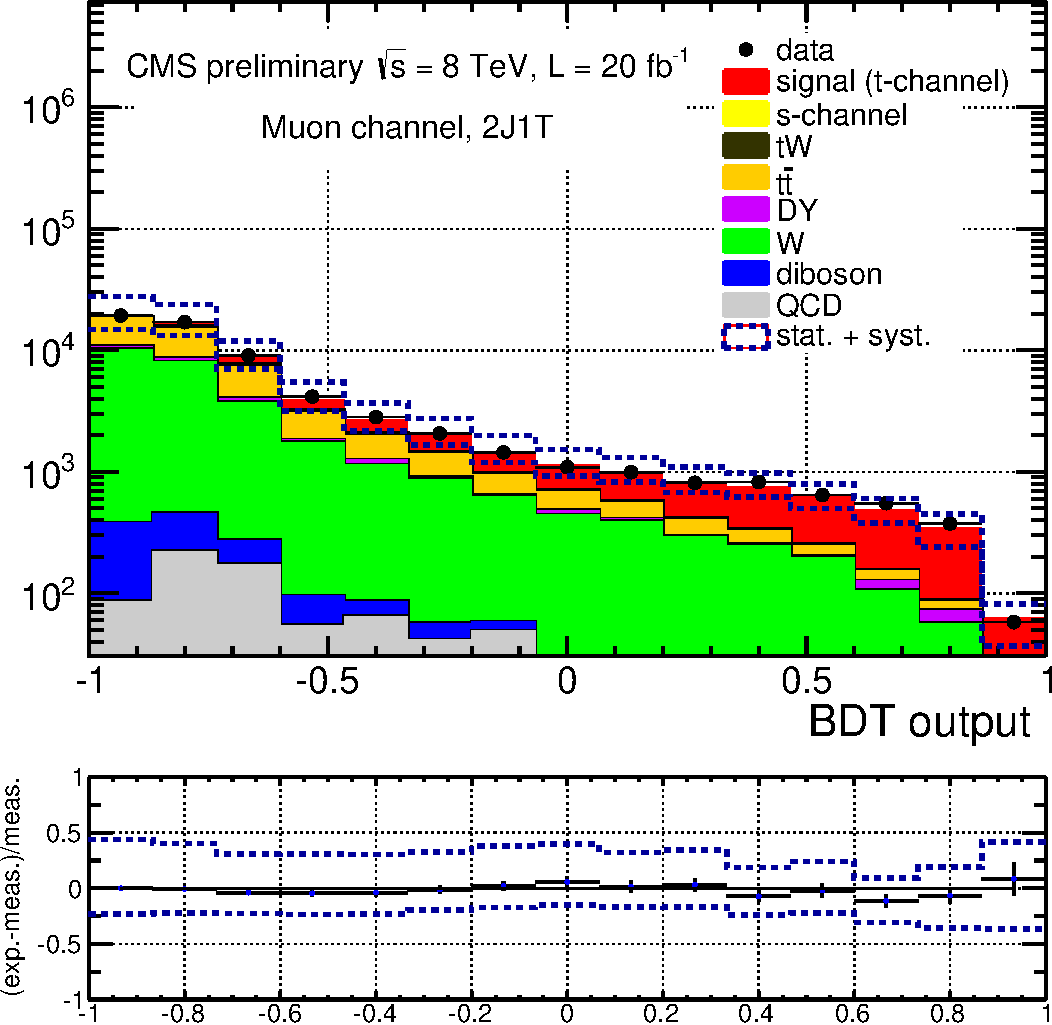
\includegraphics[height=6.5cm]{mva_bdt_mu-crop}
\center (a)
\end{minipage}\hspace{1cm}%
\begin{minipage}{7cm}
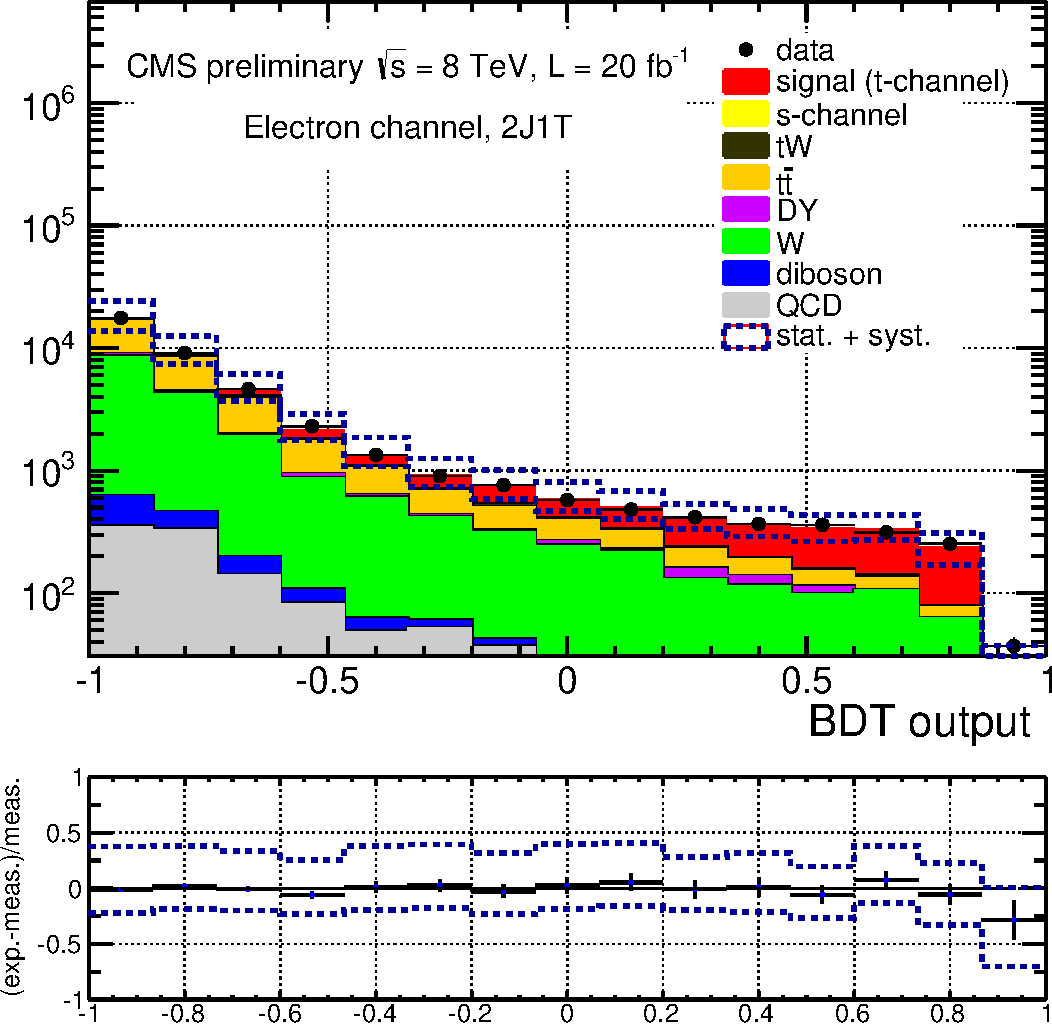
\includegraphics[height=6.5cm]{mva_bdt_el-crop}
\center (b)
\end{minipage} 
\caption{Output of the BDT trained to separate signal from $\wjets$ and $\ttbar$ in the muon (a) and electron (b) channel.}
\end{center}
\end{figure}

\begin{figure}[h]
\begin{center}
\begin{minipage}{7cm}
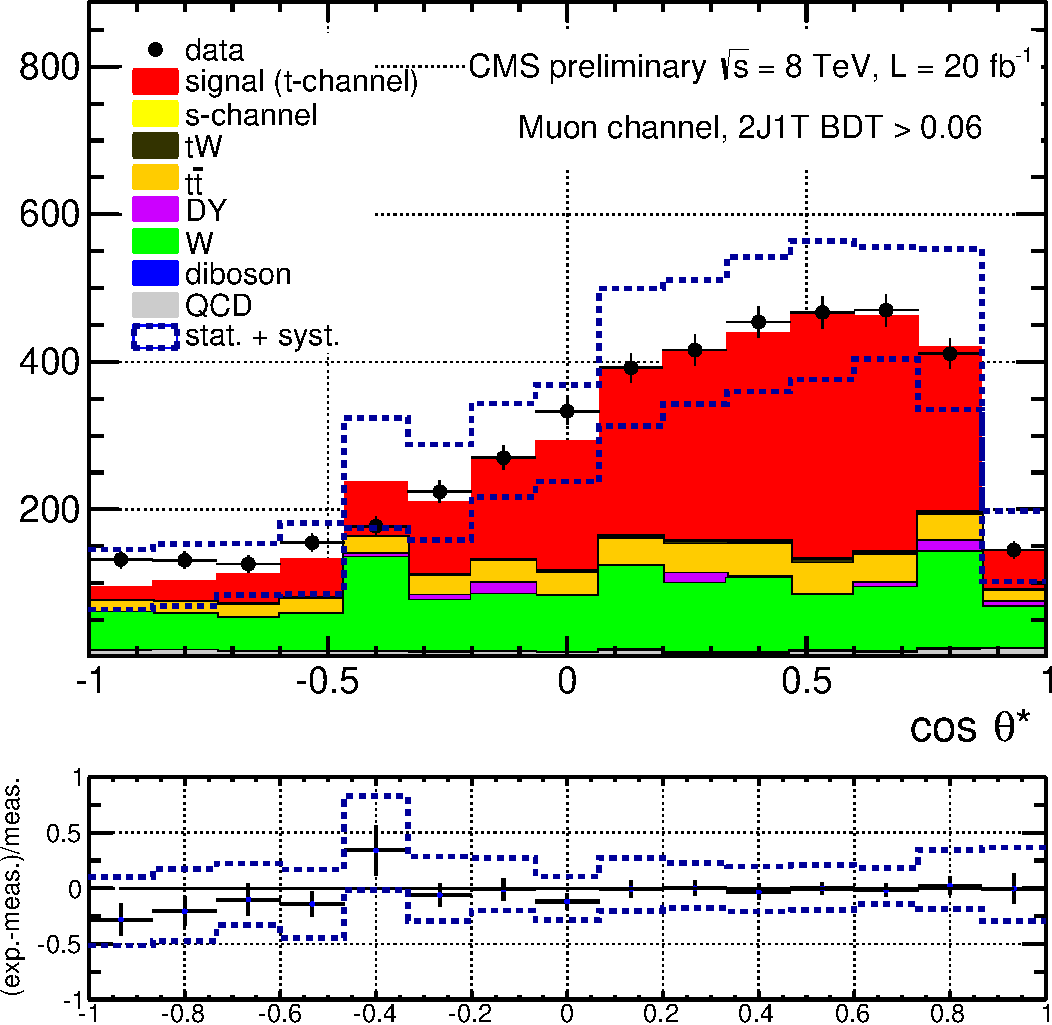
\includegraphics[height=6.5cm]{2j1t_cosTheta_mu-crop}
\caption{\label{fig:cosTheta_mu}Figure caption for first of two sided figures.}
\end{minipage}\hspace{1cm}%
\begin{minipage}{7cm}
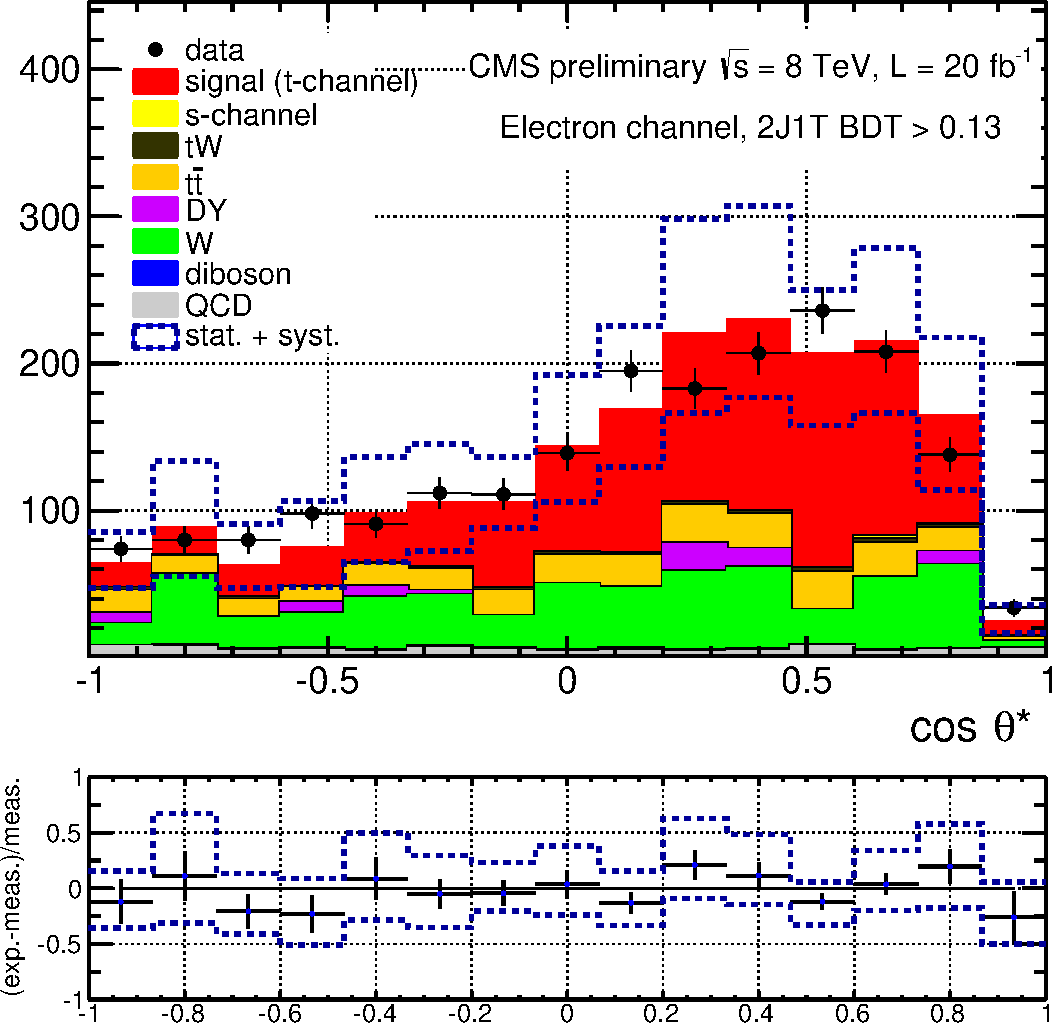
\includegraphics[height=6.5cm]{2j1t_cosTheta_el-crop}
\caption{\label{fig:cosTheta_el}}
\end{minipage} 
\end{center}
\end{figure}

\section{Unfolding}

\begin{figure}[h]
\begin{center}
\begin{minipage}{7cm}
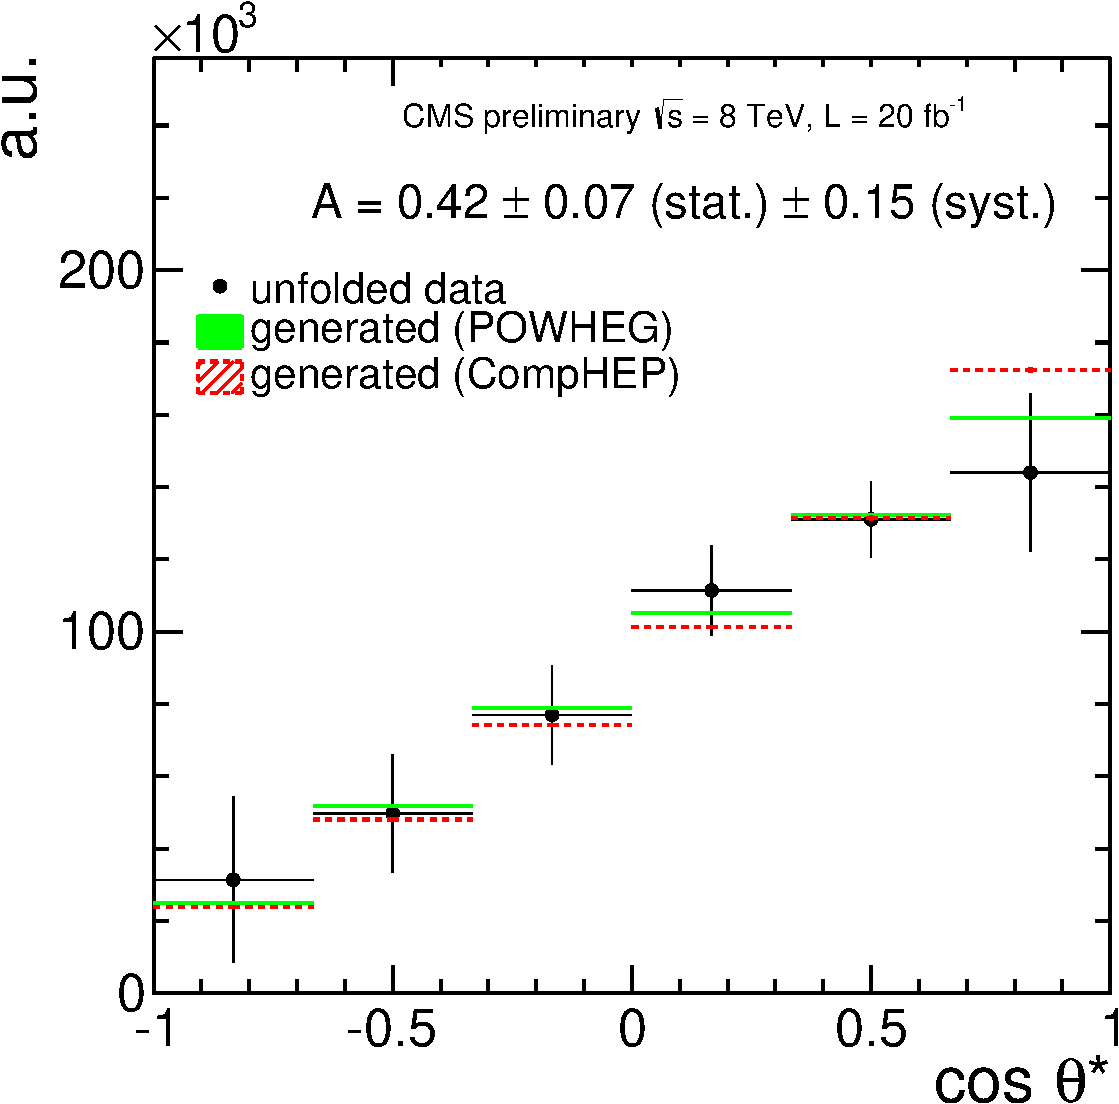
\includegraphics[height=6.5cm]{costheta_unfolded_mu-crop}
\caption{\label{fig:unfolded_mu}The unfolded $\costheta$-distribution in the muon channel.}
\end{minipage}\hspace{1cm}%
\begin{minipage}{7cm}
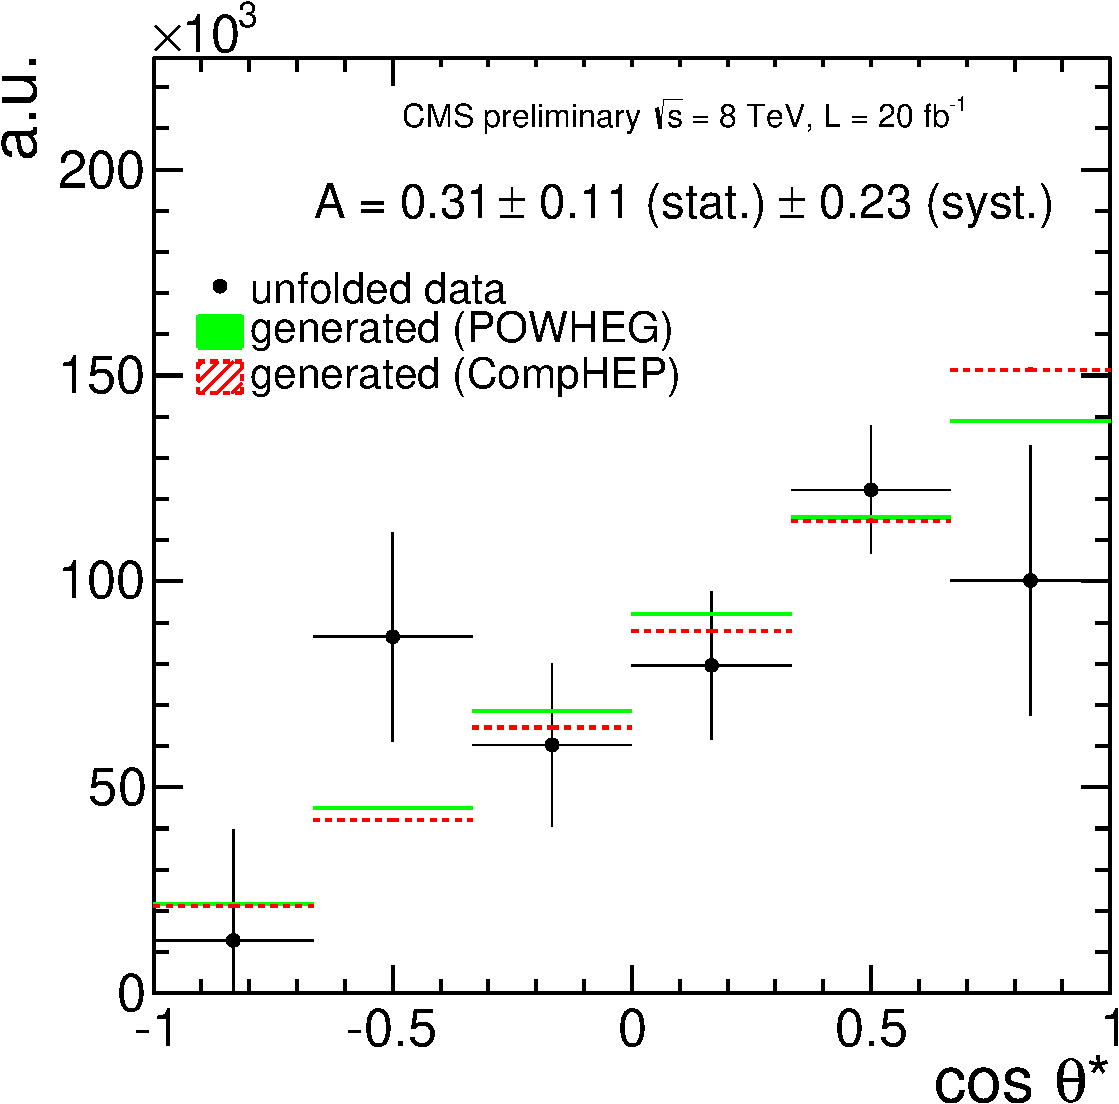
\includegraphics[height=6.5cm]{costheta_unfolded_el-crop}
\caption{\label{fig:unfolded_el}The unfolded $\costheta$-distribution in the electron channel.}
\end{minipage} 
\end{center}
\end{figure}

\section{Result}
\section{Conclusion}



\section*{References}
\begin{thebibliography}{9}
\bibitem{jaaswpol} Aguilar-Saavedra J A and Bernabeu J 2010 {\it Nucl.Phys.} {\bf B840} 349-378 
\bibitem{fabian} Bach F and Ohl T 2014 {\it Phys. Rev.} {\bf D90} 074022 



\end{thebibliography}

\end{document}


